\documentclass[12pt]{article}

% Page setup
\usepackage[a4paper, margin=1in]{geometry}

% Font
\usepackage{mathpazo}

% Formatting packages
\usepackage{setspace}
\usepackage{graphicx}
\usepackage{listings}
\usepackage{titlesec}
\usepackage{float}
\usepackage{amsmath}

% Remove page numbers
\pagenumbering{gobble}

% Line spacing
\onehalfspacing

% Code style
\lstset{
    basicstyle=\ttfamily\small,
    frame=single,
    breaklines=true,
    tabsize=2
}

% Section formatting
\titleformat{\section}{\large\bfseries}{\thesection}{1em}{}

\begin{document}
\vspace{1cm}

\section*{Experiment Name}
Write a program to compute FIRST of terminals and non-terminals of a given Context-Free Grammar (CFG).

\section*{Objective}
To compute the FIRST set for all terminals and non-terminals in a given context-free grammar (CFG). The FIRST set of a symbol $X$ is the set of terminals that appear as the first symbols in strings derived from $X$.

\section*{Algorithm}
\begin{enumerate}
    \item Start the program.

    \item Read the number of production rules from the user. For each production, read the left-hand side (non-terminal) and the right-hand side (sequence of symbols), and store them in the grammar.

    \item Identify all terminals and non-terminals from the grammar:
    \begin{itemize}
        \item Any symbol appearing on the left-hand side of a production is a \textbf{non-terminal}.
        \item Any symbol that is not a non-terminal is a \textbf{terminal} (including $\varepsilon$).
    \end{itemize}

    \item Initialize FIRST sets:
    \begin{itemize}
        \item For each terminal $a$, set $\text{FIRST}(a) = \{a\}$, since a terminal derives only itself.
        \item For each non-terminal $A$, initialize $\text{FIRST}(A) = \emptyset$ (empty set).
    \end{itemize}

    \item Apply the following fixed-point iteration — repeat until no FIRST set changes:
    \begin{itemize}
        \item For each production rule $A \rightarrow X_1\ X_2\ X_3\ \cdots\ X_n$, process each symbol $X_i$ from left to right:
        \begin{itemize}
            \item \textbf{Case 1:} If $X_1$ is a terminal $a$ (or $\varepsilon$), add $a$ (or $\varepsilon$) directly to $\text{FIRST}(A)$ and stop processing this production.
            \item \textbf{Case 2:} If $X_i$ is a non-terminal $B$, add all symbols in $\text{FIRST}(B) - \{\varepsilon\}$ to $\text{FIRST}(A)$.
            \item \textbf{Case 3:} If $\varepsilon \in \text{FIRST}(X_i)$, then $X_i$ is nullable — continue to the next symbol $X_{i+1}$ and repeat.
            \item \textbf{Case 4:} If $\varepsilon \notin \text{FIRST}(X_i)$, stop processing this production — the remaining symbols cannot contribute to $\text{FIRST}(A)$.
            \item \textbf{Case 5:} If all symbols $X_1, X_2, \ldots, X_n$ are nullable (i.e., $\varepsilon$ is in all their FIRST sets), then add $\varepsilon$ to $\text{FIRST}(A)$.
        \end{itemize}
    \end{itemize}

    \item After the iteration converges (no more changes occur), the FIRST sets are complete.

    \item Display the computed FIRST sets for all non-terminals.

    \item End the program.
\end{enumerate}
\section*{Input Grammar}
\begin{align*}
    E   &\rightarrow T\ E' \\
    E'  &\rightarrow +\ T\ E' \mid \varepsilon \\
    T   &\rightarrow F\ T' \\
    T'  &\rightarrow *\ F\ T' \mid \varepsilon \\
    F   &\rightarrow (\ E\ ) \mid \textbf{id}
\end{align*}

\newpage

\section*{Source Code}

\begin{figure}[H]
    \centering
    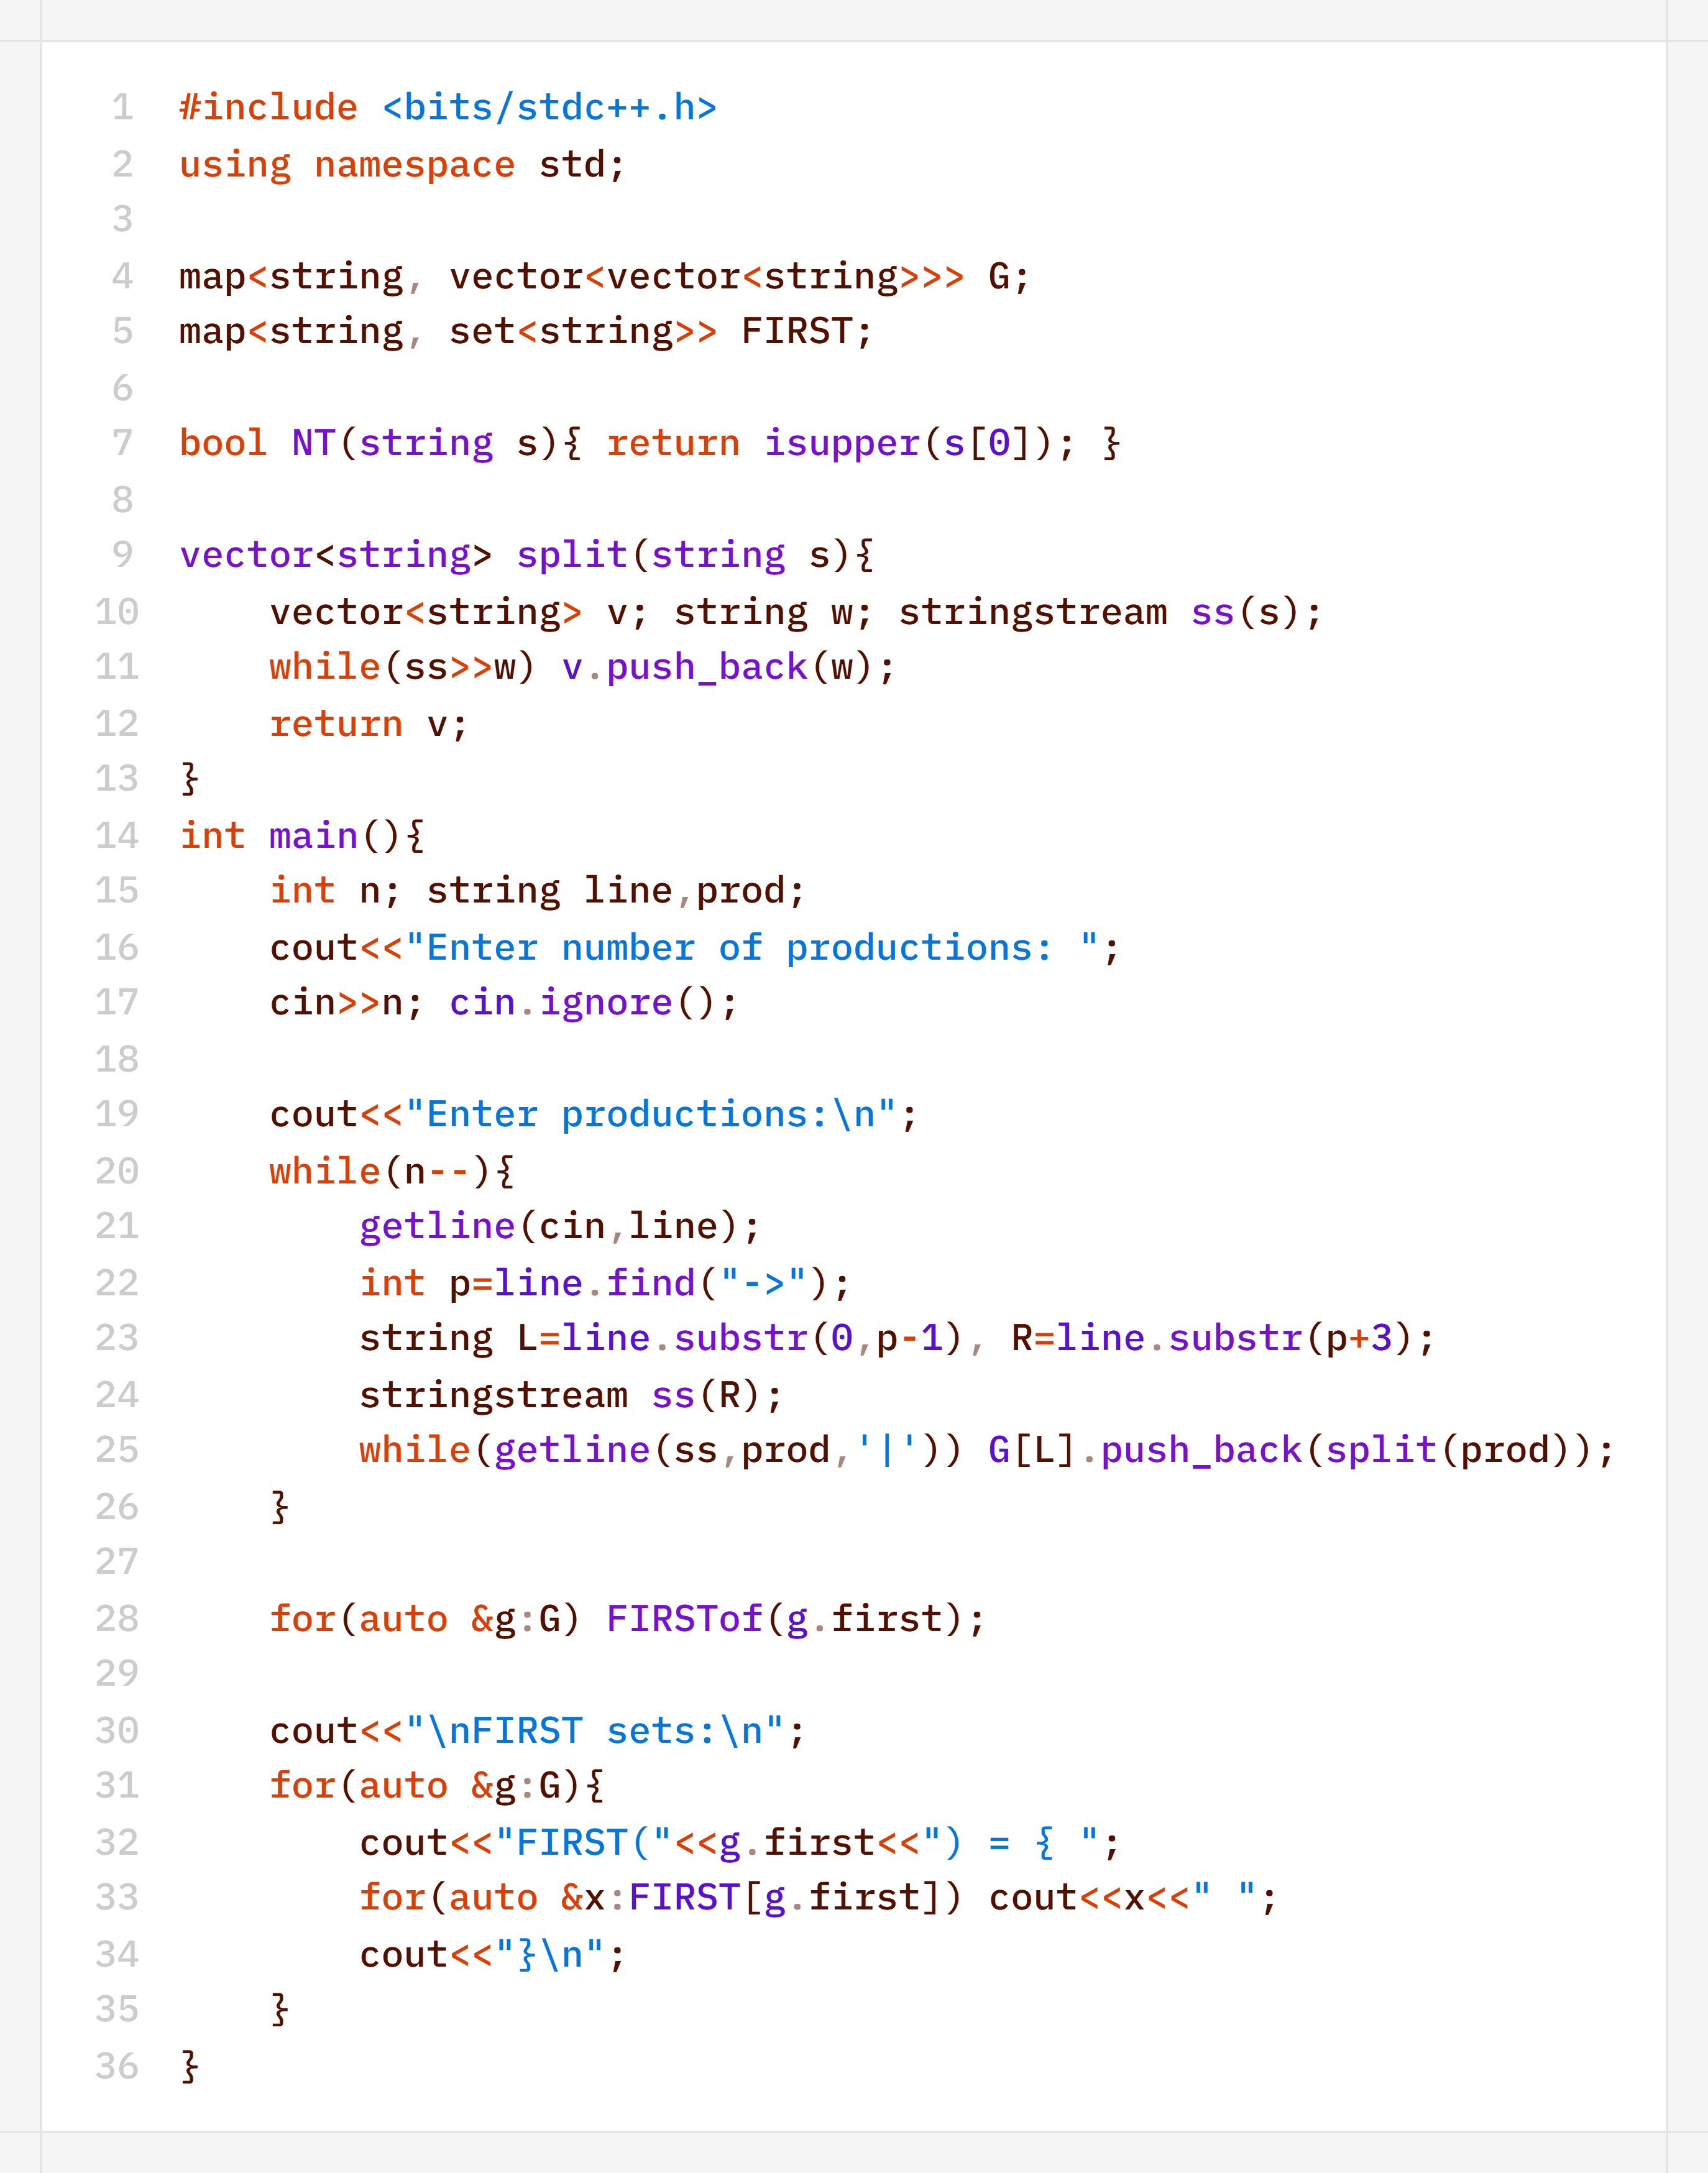
\includegraphics[width=1.0\textwidth]{source.png}
    \caption{Source code for computing FIRST sets of a given grammar}
\end{figure}


\section*{Output Screenshot}

\begin{figure}[H]
    \centering
    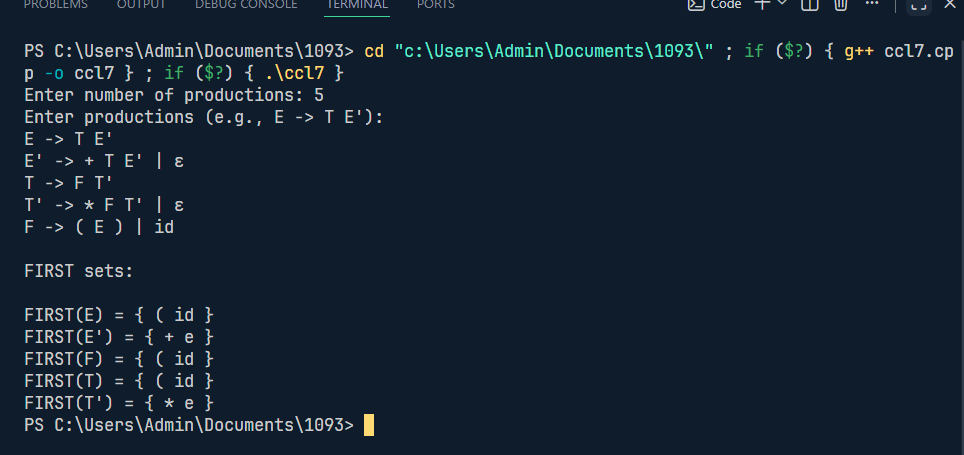
\includegraphics[width=0.85\textwidth]{output_ss.png}
    \caption{Output showing computed FIRST sets}
\end{figure}


\section*{Discussion}
This experiment demonstrates the implementation of the FIRST set computation algorithm for context-free grammars. The FIRST set is a fundamental concept in compiler construction, particularly used in the design of top-down parsers such as the LL(1) parser.

The program correctly handles all cases: productions starting with a terminal (directly added to the FIRST set), productions starting with a non-terminal (FIRST of that symbol minus $\varepsilon$ is propagated), nullable non-terminals (algorithm looks ahead to the next symbol), and epsilon productions (added when all symbols in a production are nullable).

\end{document}